\subsection{Blockchain}
Blockchain\cite{Bitcoin2015,blockchain-hype,blockchain-tech} is a type of \acrfull{dlt} which provides several properties. The main ones, known as the three pillars of the blockchain technology are:
\begin{itemize}
    \item \textbf{Decentralization}. The information is not stored by a single entity, in fact, everyone in the network owns the information and can access it. Decentralization means that there is no core authority to dictate the truth to the other participants. Also, in a decentralized network, if you want to interact with another participant, you can do it directly without going through a third party.
    \item \textbf{Transparency}. The most misunderstood property. Some people say blockchain gives you privacy while some say that it is transparent. The fact is, that blockchain technology gives you both. Transparency because every participant in the network can see the transactions and its data, and privacy because the involved accounts are hidden via complex cryptography. In the figure below (figure \ref{fig:alastria_block_explorer}) we can see the public transaction in the Alastria network, but we are not able to know the accounts "from" and "to".
          \begin{figure}[h]
              \centering
              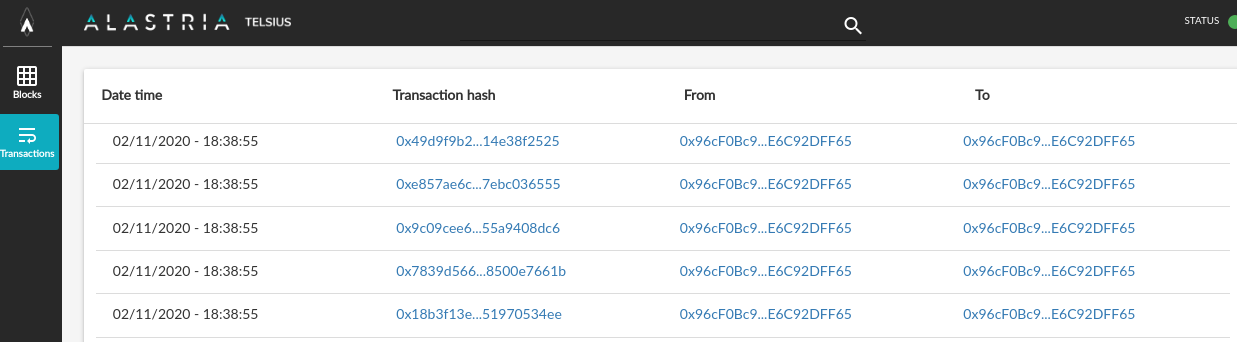
\includegraphics[width=1.1\textwidth]{Alastria-block-exporer.png}
              \caption{Alastria's Block explorer}
              \label{fig:alastria_block_explorer}
          \end{figure}
    \item \textbf{Immutability}. This property ensures that once something has been entered into the blockchain, it cannot be tampered or modified.
\end{itemize}

\subsubsection{How does Blockchain work?}
A Blockchain is a growing list of records, called blocks (figure \ref{fig:linked_blocks}), that are linked using cryptography. Each block contains a hash of the previous block, the timestamp and a batch of valid transaction hashes encoded into a Merkle tree. The linked blocks form a chain. This iterative process confirms the integrity of the previous block, all the way back to the original genesis block (the first block of the network).
\begin{figure}[h]
    \centering
    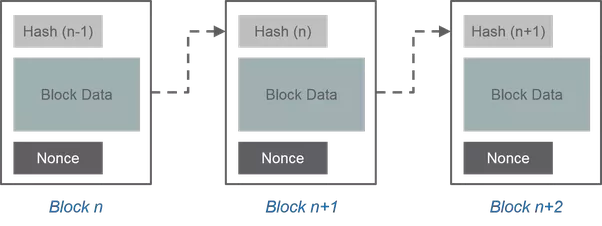
\includegraphics[width=1.0\textwidth]{block-example.png}
    \caption{Visual example of linked blocks}
    \label{fig:linked_blocks}
\end{figure}

\subsubsection{Types of blockchains}
There are different kinds of Blockchain networks, each one with different features (figure  \ref{fig:blockchain_classification}). One of the most common classification is according to the architecture. The following figure shows a table with the classification.
\begin{figure}[h]
    \centering
    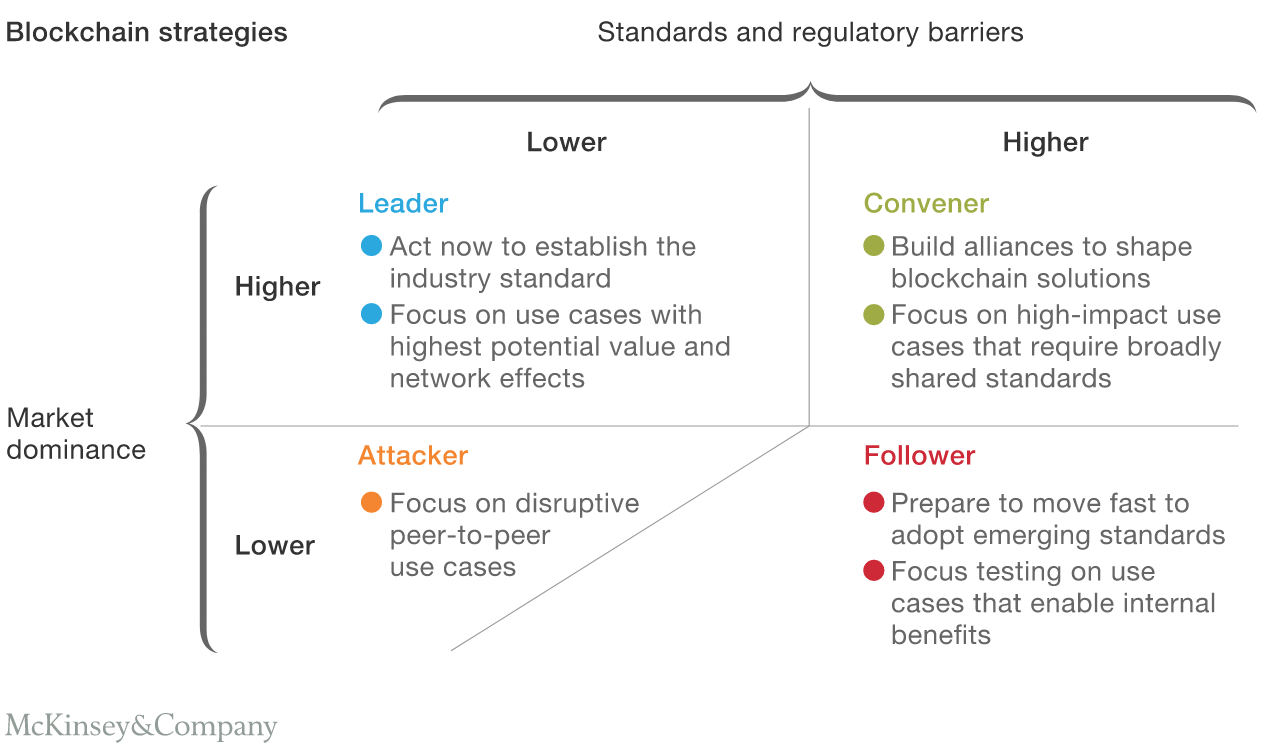
\includegraphics[width=1.0\textwidth]{Blockchain-types.png}
    \caption{Blockchain architecture classification by \textit{McKinsey\&Company}}
    \label{fig:blockchain_classification}
\end{figure}

\begin{itemize}
    \item \textbf{Public}. A public network is the one where everyone can join. Some examples of public networks are Bitcoin, Ethereum and Litecoin.
    \item \textbf{Private}. A private network is the one where only authorized members can join. Some examples of private networks are Quorum and Monax.
    \item \textbf{Permissionless}. A permissionless network is a private or public blockchain where every member can read and write.
    \item \textbf{Permissioned}. A permissioned network is a private or public blockchain where every member can read but only some can write. Some examples of public permissioned networks are Alastria and LACChain.
\end{itemize}
Also, there are two more types of blockchain networks on the rise.
\begin{itemize}
    \item \textbf{Consortium} or \textbf{hybrid networks}. These networks are private and permissioned, operated by known entities such as stakeholders of a given industry regrouped in a consortium or exploiting a shared platform. Some known examples are \textit{Hyperledger} \textit{Fabric}, \textit{R3 Corda} and \textit{Multichain}.
    \item \textbf{\acrfull{baas}}. These are cloud platforms hosted by a service provider to deploy blockchain applications. The service provider manages the blockchain network while the customer defines the business logic. Some of the examples are \textit{\acrfull{aws}} and \textit{Oracle} blockchain platforms.
\end{itemize}

\subsubsection{Uses of blockchain}
With the different properties of blockchain technology, and the different types of networks, there are a lot of use cases (figure \ref{fig:blockchain_uses}). The best known use case is using the blockchain as a payment infrastructure, the best example is Bitcoin. But there are a lot of other use cases shown in the next figure.\\
\begin{figure}[h]
    \centering
    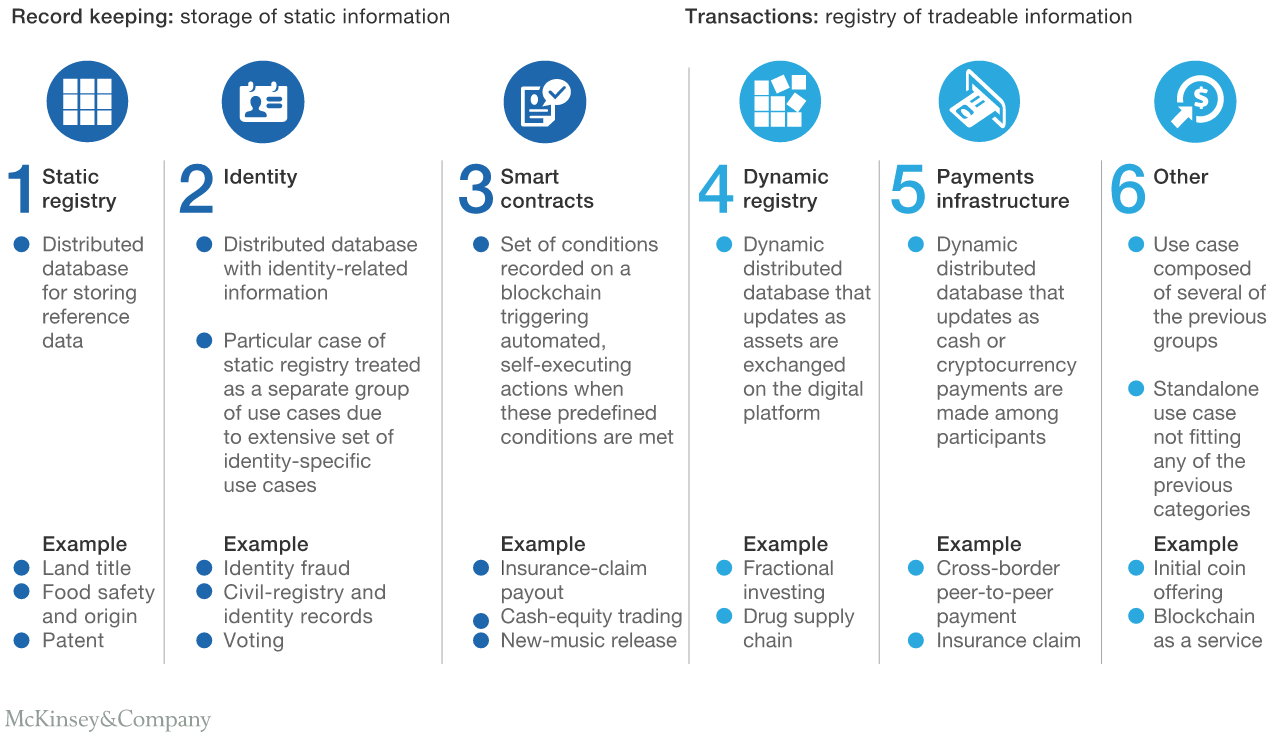
\includegraphics[width=0.95\textwidth]{Blockchain-uses.png}
    \caption{Blockchain use cases table by \textit{McKinsey\&Company}}
    \label{fig:blockchain_uses}
\end{figure}

In this document we are going to focus on the \acrfull{ssi} using blockchain.
